\startchapter{Methods} \label{ch:2}
\section{Current Approaches to Molecular Structure Elucidation}
Currently, there are two main approaches in studying the orientation distribution of molecules at interface. One is comparing the experimental spectra with few predicted ones, and select the one that most matches to the experimental one. Another one is running an exhaustive algorithm to explore the most possible solution space \cite{hore0033-rotations}. However, both approaches take a lot of time and computational resources. In Hung's study \cite{KuoKaiHung:Thesis:2015}, a new approach is introduced. He applied LP to vibrational spectra to extract the molecular structure at interfaces. This LP approach helped to return the target orientation distribution information when the mock experimental spectrum consisted of different amino acids. However, when candidates are coming from the same amino acid, LP approach failed to return the target orientation distribution information. The reason why LP failed to return the target composition has not been thoroughly studied in Hung's study. Whether and how LP approach can be generally applied to different experiment situations have not been explored. My study is to figure out the underlying properties of our LP model. Furthermore, explore the applicability of the LP model to different experimental setting. \\
	
\section{Structure of molecules adsorbed to interfaces}
(TODO: check with Dennis, how to expand this part.) A picture to display molecules adsorbed to interfaces


\section{Generating model spectra}
As mentioned in Chapter \ref{ch:1}, before analyzing the vibrational spectra of amino acids, there are a few factors to address. First of all, creating candidate spectra is an essential step. This part of research has been done thoroughly by Hung \cite{KuoKaiHung:Thesis:2015}. \\

To generate these amino acids' vibrational spectra, a molecule's vibration modes need to be modelled in the molecular frame, then transferred to the laboratory frame to work with the systems where interfaces exist. Chapter 2 in Hung's thesis \cite{KuoKaiHung:Thesis:2015} describes how to perform electronic structure calculations using GAMESS \cite{GAMESS} to obtain the derivatives of every dipole moment and polarizability. Then he introduced how to use Direction Cosine Matrix (DCM) to transfer these two derivatives from the molecular coordinate system to the laboratory one. After that, Euler angles could be extracted from DCM. Euler angles are used to describe a molecule's coordination at interfaces. They are labelled by $\theta$, $\phi$ and $\psi$ as shown in Figure \ref{fig:2.1}. They are referred as $tilt$, $azimuthal$ and $twist$ angles, respectively. Let $x$, $y$ and $z$ be lab frame Cartesian coordinates, and $a$, $b$ and $c$ be the molecular frame coordinates. $Tilt$ angle $\theta$ is the angle between $z$ and $c$. $Azimuthal$ angle $\phi$ is the rotation about $z$. $Twist$ angle $\psi$ is a twist about $c$ \cite{hore0033-rotations}. After three steps of successive rotations of Euler angles, molecule properties can be transferred from the molecular frame to the lab frame. \\

In order to achieve the above steps, Hung first did a Hessian calculation using GAMESS. Secondly, 7 snapshots of a molecule vibrating in different modes were taken. Thirdly, he did a force field calculation to obtain the derivatives of dipole moment and polarizability for each 7 snapshot moment. Then the derivatives of dipole moment and polarizability are obtained by the interpolation of these 7 snapshot moment. Because the two obtained derivatives are in the molecular frame, Hung used DCM to convert these two derivatives into the lab frame. Then abstracted Euler angles from DCM. After this transformation, he restored the derivatives information into some molecular property files for any further usage. (TODO: double check the accuracy with Dennis)\\

\begin{figure}[!ht] 
\centering
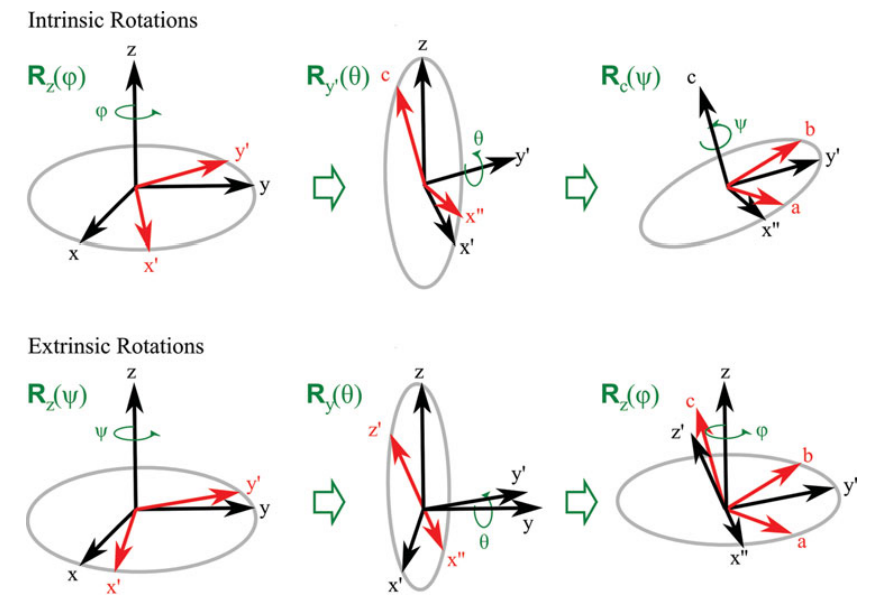
\includegraphics[scale=0.5]{Figures/Euler_angles_represented_as_the_spherical_polar_angles.png} 
\caption{The Euler angles represented as the spherical polar angles $\theta$, $\phi$ and $\psi$, and the illustration of the three successive rotations that transform the lab $x$, $y$, $z$ coordinate system into the molecular $a$, $b$, $c$ frame intrinsically and extrinsically \cite{hore0033-rotations}. }
\label{fig:2.1}
\end{figure}

In my study, those molecular property files are used to generate the amino acids' spectroscopy information directly. Each molecular property file contains the derivatives of dipole moment and polarizabilities of each vibrational mode. Depends on the number $N$ of atoms in a molecule, there are $3N-6$ vibrational modes. Furthermore, Equation \ref{eq:2.2} to \ref{eq:2.4} are used to generate the amino acids' IR, Raman and SFG spectra. \\

All the experiments in my study are limited to only consider the $tilt$ angle distribution of Euler angles, and assume isotropy on $twist$ and $azimuthal$ angular distributions. Therefore, $twist$ and $azimuthal$ angles are integrated to create a uniform distribution. For angle $\psi$, it requires the surfaces to be not striped. There can be no anisotropy in the plane of the surface. Because of this, we can limit the candidate number by integrating angle $\psi$. On the other hand, for angle $\phi$, a uniform distribution implies that the molecule has cylindrical symmetry in its preference of surface. This means that the molecule can be tilted, but has no `twist' preference. With the integration of these two Euler angles, the number of candidates for one molecule will be greatly reduced. However, the number of the amino acid candidates is still large when only considering $\theta$ angle. The possible combinations of all these amino acid candidates are still considered to be excessive (TODO: put these into an approximated number???). \\

Furthermore, when molecules lay on an interface, the orientation of each molecule varies. To simulate the vibrational spectra, a reasonable orientation distribution for the molecules needed to be studied. The orientation distribution requires either do a molecular dynamic simulation to study the distribution of molecule orientations at the interface, or come up with a analytic orientation distribution function. In my study, the second method is preferred. Moreover, Delta distribution function shown in Equation \ref{eq:2.1} is used to represent the molecule orientation distribution that models the spectrum signals. This means that all the molecules are tilted at one same angle at the interface. This assumption is applied across the whole study. \\
\begin{equation} \label{eq:2.1}
f_{(\theta)} = \delta(\theta - \theta_{o})
\end{equation} 

Infrared (IR) absorption spectroscopy is a harmonic approximation, its intensity is proportional to the square of the lab-frame dipole moment derivative. For example, the $x$-polarized absorption spectrum is given by Equation \ref{eq:2.2}. \\

\begin{equation} \label{eq:2.2}
I_x(\omega_{\rm IR}) = \sum_{q} \frac{1}{2 m_{q} \omega_{\rm q}} \Bigg \langle \Bigg\lbrack \frac{\partial u_x}{\partial Q} \Bigg\rbrack_{q} ^2 \Bigg\rangle \frac{\Gamma_q^2}{(\omega_{\rm IR}-\omega_{\rm q})^2 + \Gamma_q^2}
\end{equation} 
where $I_x$ represents $x$-polarized intensity. The same equation applies to $I_y$ and $I_z$. $\omega_{\rm IR}$ is the frequency of the probe radiation. $\mu$ is the dipole moment. $m_q$ is the reduced mass. $w_q$ is resonance frequency. $\Gamma_q$ is the homogeneous line width, is set to 6 in all the experiments. $Q_q$ is the normal mode coordinate of the $q$th vibrational mode. All values of $\omega_{\rm IR}$, $\mu$, $m_q$, $Q$ are obtained from the molecular property files. Furthermore, because $\phi$ and $\psi$ angles are integrated, the $y$-polarized spectrum is identical with the $z$-polarized one. Therefore, there are only two unique polarized IR spectra. For simplicity, IR spectra are referred as $y$ and $z$ in future experiments.(TODO: need to double check the accuracy with Dennis) \\

The intensity of Raman scattering is proportional to the square of laboratory-frame transition polarizability. For example, Raman spectroscopy with an $x$-polarized excitation source collects the $x$-polarized component of the scattered radiation, which can be approximated from Equation \ref{eq:2.3}. \\

\begin{equation} \label{eq:2.3}
I_{xx}(\Delta \omega) = \sum_{q} \frac{1}{2 m_{q} \omega_{\rm q}} \Bigg \langle \Bigg\lbrack \frac{\partial \alpha_{xx}^{(1)}}{\partial Q} \Bigg\rbrack_{q} ^2 \Bigg\rangle \frac{\Gamma_q^2}{(\Delta \omega-\omega_{\rm q})^2 + \Gamma_q^2}
\end{equation} 
where $\Delta w$ is the Stokes Raman shift. $\alpha_{xx}^{(1)}$ is one component of the $9$-element polarizability tensor. $m_q$, $w_q$, $\Gamma_q$, and $Q_q$ are the same as defined above for IR spectra. All the values of $\omega_{\rm IR}$, $\mu$, $m_q$, $Q$ are obtained from the molecular property files. Similar to IR spectroscopy, because of the integration of $\phi$ and $\psi$ angles, only 4 unique spectra are obtained from the following polarization: $xx$, $xy$, $xz$ and $zz$. For simplicity, Raman spectra are referred as $xx$, $xy$, $xz$ and $zz$ in future experiments (TODO: double check the accuracy of the content with Dennis). \\

The intensity of SFG spectroscopy is proportional to the squared magnitude of the second-order susceptibility, $\left|\chi^{(2)}\right|^{2}$. $\chi^{(2)}$ is derived from the second-order polarizability, $\alpha^{2}$. Equation \ref{eq:2.4} shows the response intensity of $I_{xxx}$. \\
\begin{equation} \label{eq:2.4}
I_{xxx}(\omega_{\rm IR}) = \sum_{q} \frac{1}{2 m_{q} \omega_{\rm q}} \Bigg \langle \Bigg\lbrack \frac{\partial \alpha_{xx}^{(1)}}{\partial Q} \Bigg\rbrack_{q} \Bigg\lbrack \frac{\partial u_{x}}{\partial Q} \Bigg\rbrack_{q} \Bigg\rangle \frac{1}{\omega_{\rm q}-\omega_{\rm IR}-i\Gamma_q}
\end{equation} 
where $I_{xxx}$ is the second-order susceptibility tensor. It is probed by an $x$-polarized visible incoming beam at frequency $\omega_{\rm vis}$ and a $x$-polarized infrared beam incoming with frequency $\omega_{\rm IR}$. Both incoming beams are incident to the sample. Then the $x$-component of SFG at frequency $\omega_{SFG}=\omega_{\rm vis}+\omega_{\rm IR}$ is selected for detection. As $i=\sqrt{-1}$ is in the denominator, $X^{(2)}$ is a complex value \cite{KuoKaiHung:Thesis:2015}. The SFG response is the imaginary component of the second-order susceptibility. Same as IR and Raman spectroscopy, all the values of $\omega_{\rm IR}$, $\mu$, $m_q$, $Q$ are obtained from the molecular property files. Because of the integration of $\phi$ and $\psi$ angles, only 3 unique non-zero spectra are obtained from the following polarizations: $yyz$, $yzy$ and $zzz$. For simplicity, SFG spectra are referred as $yyz$, $yzy$ and $zzz$ in future experiments.  (TODO: double check the accuracy of the content with Dennis). \\

With these equations and the molecular property files, IR, Raman and SFG spectra can be generated for a candidate. A candidate in my study is a specific amino acid with specific $\theta$ value. Taking Methionine as an example, Figure \ref{fig:2.2} displays $x$-polarized IR spectra of the following candidates: Methionine with $\theta$ of $0^{\circ}$, $20^{\circ}$, $40^{\circ}$ and $60^{\circ}$. Their spectra are prefixed with $candidate\_$ in the labels. $ir\_x\_$ indicates the spectroscopy technique, ``number" indicates the $\theta$ angle's value. The spectra labelled as $target\_ir\_x$, is generated by combining $10\%$ of $candidate\_ir\_x\_0$, $50\%$ $candidate\_ir\_x\_20$ and $40\%$ $candidate\_ir\_x\_40$. \\

Similarly, Figure \ref{fig:2.3}, \ref{fig:2.4} and \ref{fig:2.5} depict the spectra of the same candidates and targets for $z$-polarized IR, $xx$-polarized Raman and $yyz$-polarized SFG spectrum respectively. In Figure \ref{fig:2.2}, the biggest differences among the candidates exist at each vibrational mode. The valid range for wavenumber is from 1000 to 2000. Each polarization of IR, Raman or SFG, there are 200 data points can be extracted in the interval of 5 wavenumber. With these data points, the corresponding LP model is constructed as described in Chapter \ref{ch:3}.\\

\begin{figure}[!ht]
\centering
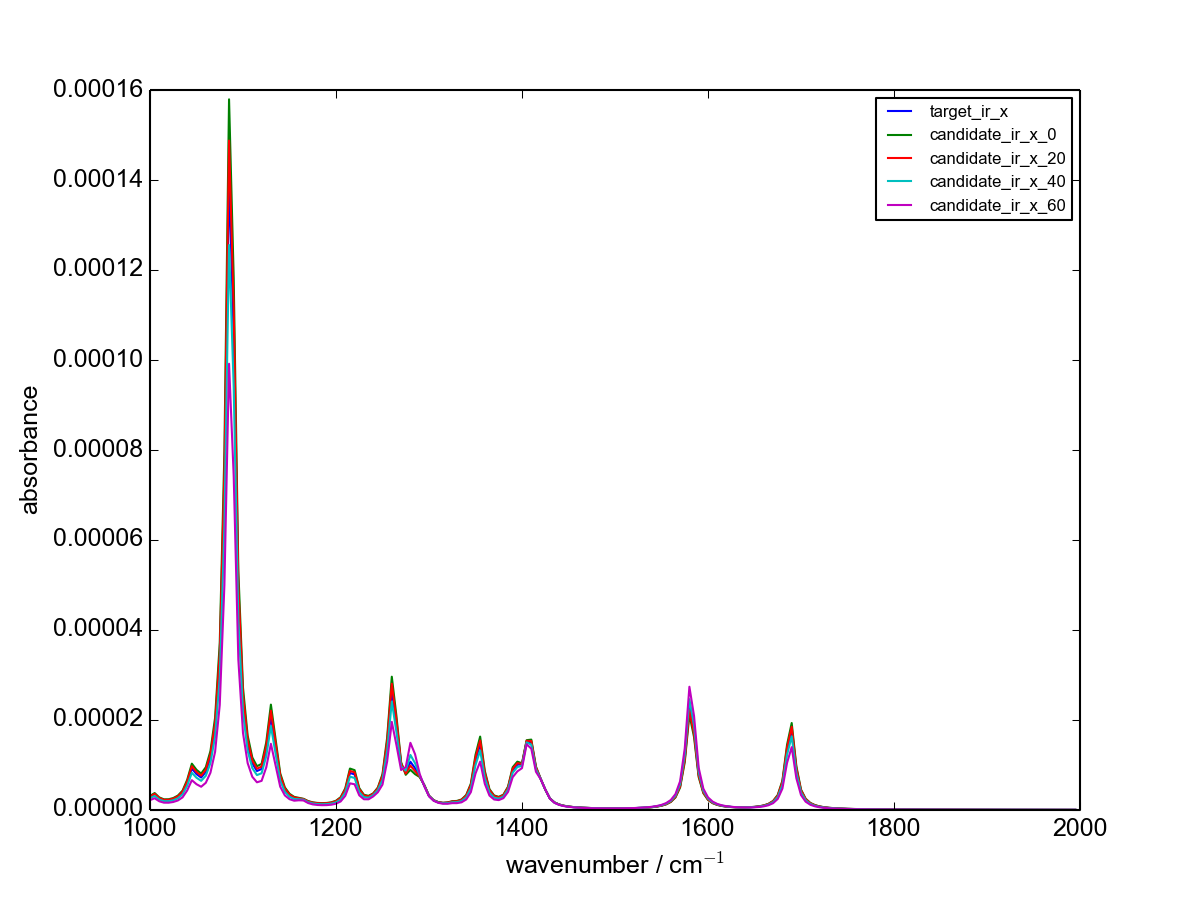
\includegraphics[scale=0.5]{Figures/Met_candidates_plotting_ir_x.png}
\caption{IR $x$-polarized spectra of methionine's four candidates and target. The candidates are with $\theta$ of $0^{\circ}$, $20^{\circ}$, $40^{\circ}$ and $60^{\circ}$. The target is produced by combining $10\%$ of $candidate\_ir\_x\_0$, $50\%$ $candidate\_ir\_x\_20$ and $40\%$ $candidate\_ir\_x\_40$. } \label{fig:2.2}
\end{figure}

\begin{figure}[!ht]
\centering
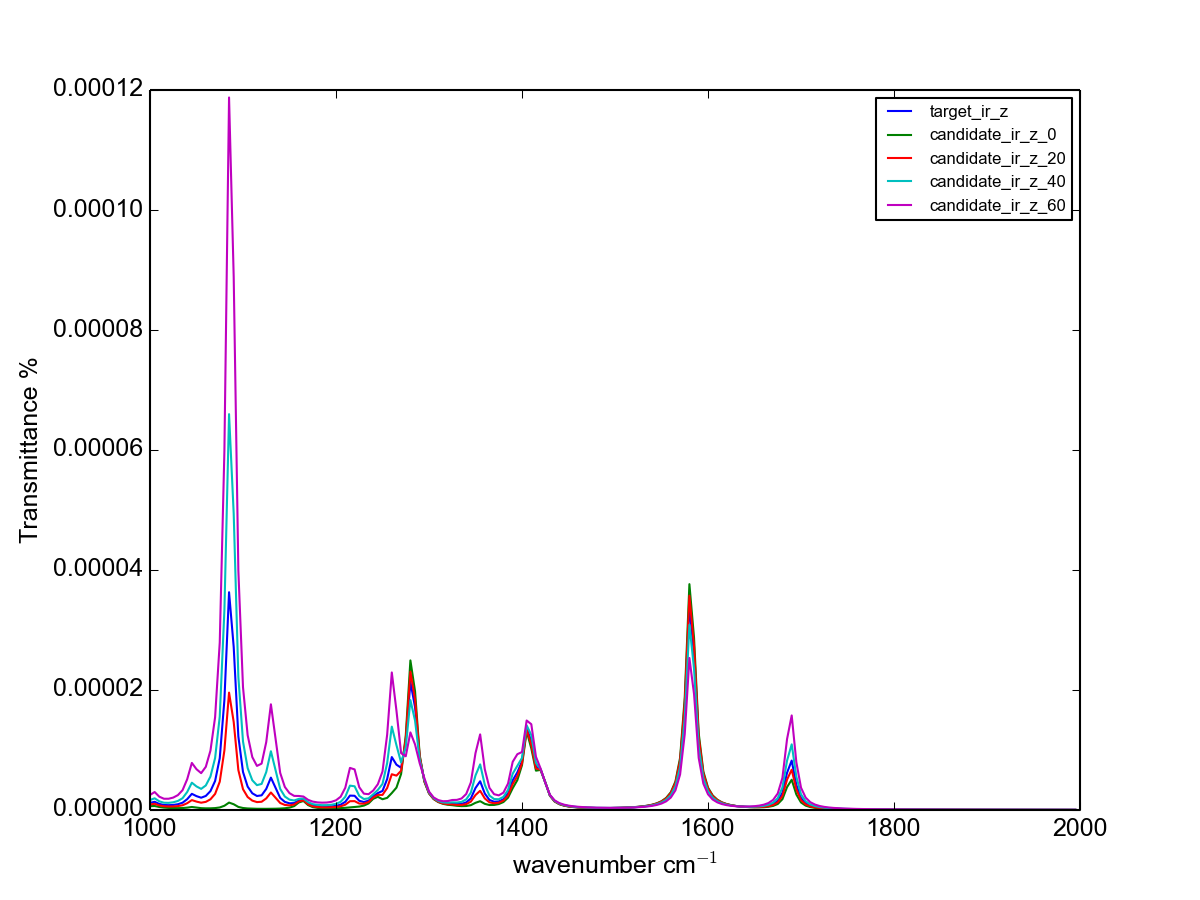
\includegraphics[scale=0.5]{Figures/Met_candidates_plotting_ir_z.png}
\caption{IR $z$-polarized spectra of methionine's four candidates and target. The candidates are with $\theta$ of $0^{\circ}$, $20^{\circ}$, $40^{\circ}$ and $60^{\circ}$. The target is produced by combining $10\%$ of $candidate\_ir\_x\_0$, $50\%$ $candidate\_ir\_x\_20$ and $40\%$ $candidate\_ir\_x\_40$.} \label{fig:2.3}
\end{figure}

\begin{figure}[!ht]
\centering
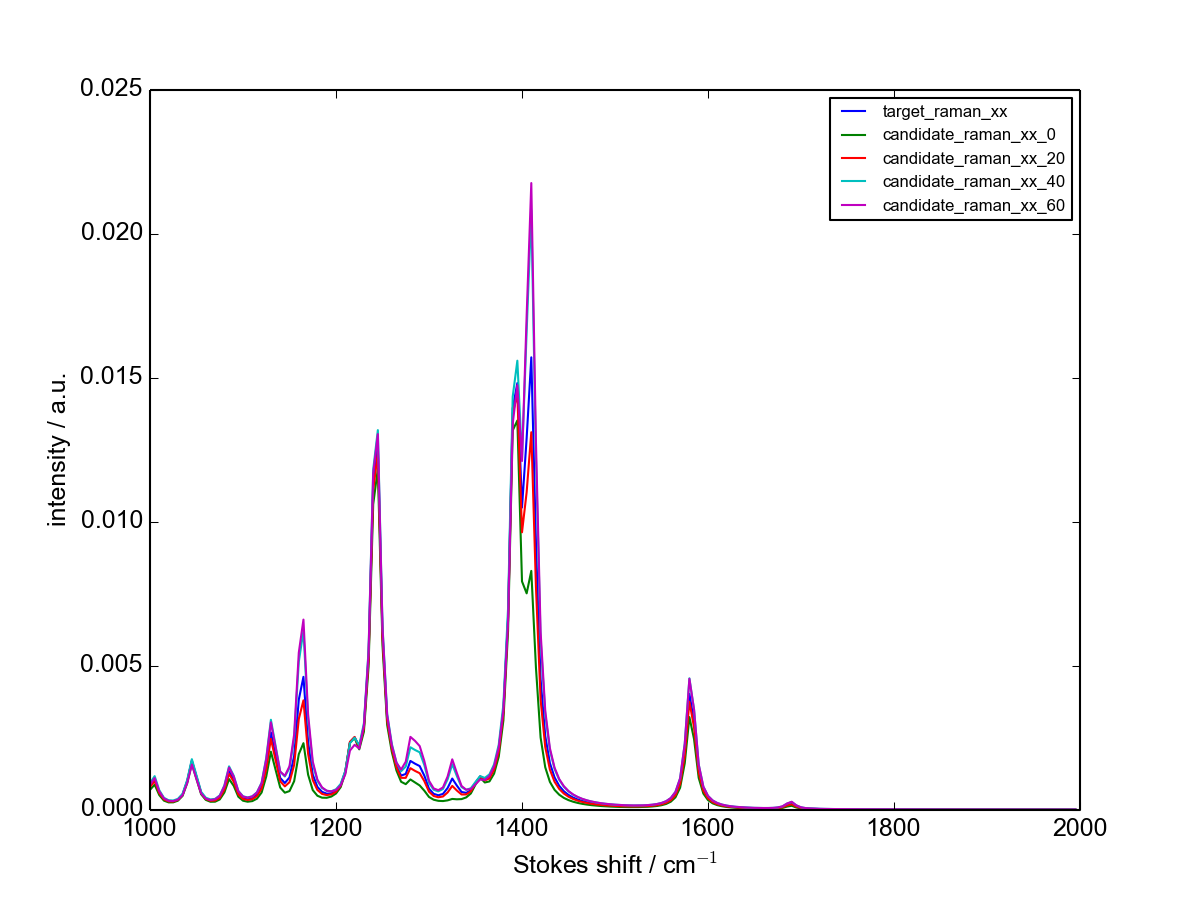
\includegraphics[scale=0.5]{Figures/Met_candidates_plotting_raman_xx.png}
\caption{Raman $xx$-polarized spectra of methionine's four candidates and target. The candidates are with $\theta$ of $0^{\circ}$, $20^{\circ}$, $40^{\circ}$ and $60^{\circ}$. The target is produced by combining $10\%$ of $candidate\_ir\_x\_0$, $50\%$ $candidate\_ir\_x\_20$ and $40\%$ $candidate\_ir\_x\_40$.} \label{fig:2.4}
\end{figure}

\begin{figure}[!ht]
\centering
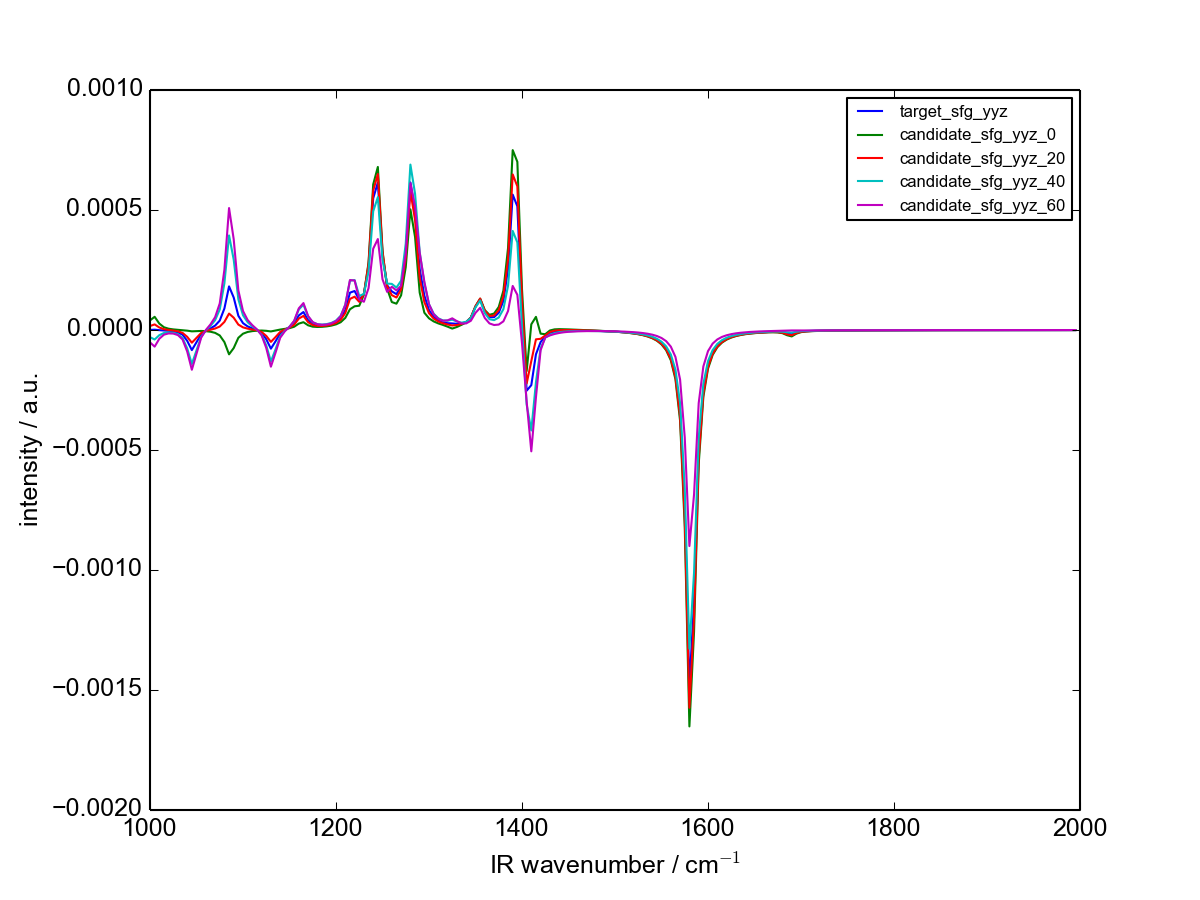
\includegraphics[scale=0.5]{Figures/Met_candidates_plotting_sfg_yyz.png}
\caption{SFG $yyz$-polarized spectra of methionine's four candidates and target. The candidates are with $\theta$ of $0^{\circ}$, $20^{\circ}$, $40^{\circ}$ and $60^{\circ}$. The target is produced by combining $10\%$ of $candidate\_ir\_x\_0$, $50\%$ $candidate\_ir\_x\_20$ and $40\%$ $candidate\_ir\_x\_40$.} \label{fig:2.5}
\end{figure}

\section{The Properties of the LP Models}
Chapter \ref{ch:2} explains what are the current approaches to extract molecular structure at interfaces, and how to produce IR, Raman and SFG spectra theoretically. In Chapter \ref{ch:3}, the properties of the LP model are studied. It is conducted by using a toy model to gain an insight of the behaviours our LP approach. The motivation of creating a toy model is to create a molecule as simple as possible, so that only the properties of the LP model is focused. With the further information gained in Chapter \ref{ch:3}, further experiences will be conducted to real molecules in Chapter \ref{ch:4}, \ref{ch:5} and \ref{ch:6}.